\documentclass[11pt,a4paper]{article}

\usepackage[margin=1in]{geometry}
\usepackage{graphicx}
\usepackage{xcolor}
\usepackage{titlesec}
\usepackage{enumitem}
\usepackage{hyperref}
\usepackage{fancyhdr}
\usepackage{float}

\definecolor{brandindigo}{HTML}{4F46E5}
\definecolor{brandamber}{HTML}{F59E0B}
\definecolor{brandgray}{HTML}{4B4B57}

\titleformat{\section}{\normalfont\Large\bfseries\color{brandindigo}}{\thesection}{1em}{}
\titleformat{\subsection}{\normalfont\large\bfseries\color{brandgray}}{\thesubsection}{1em}{}

\pagestyle{fancy}
\fancyhf{}
\fancyhead[L]{VenueLock --- App Description}
\fancyhead[R]{\thepage}
\renewcommand{\headrulewidth}{0.4pt}

\hypersetup{
    colorlinks=true,
    linkcolor=brandindigo,
    urlcolor=brandindigo,
}

\title{\textbf{\Huge VenueLock} \\[0.3em] \Large Every Seat, Accounted For \\[0.5em] \normalsize App Description}
\author{}
\date{}

\begin{document}

\maketitle
\thispagestyle{empty}

\begin{center}

\includegraphics[width=0.28\textwidth]{screenshots/app_icon.png}
\end{center}

\vspace{1em}

\begin{center}
\begin{minipage}{0.85\textwidth}
\itshape\centering
Cap attendance at an exact seat count --- book a seat, get a QR pass,
scan in.
\end{minipage}
\end{center}

\newpage

% ─────────────────────────────────────────────────────────────
\section{At a Glance}

\begin{itemize}[leftmargin=1.5em]
    \item \textbf{App name:} VenueLock
    \item \textbf{Category:} Events / Productivity
    \item \textbf{Platforms:} Android, iOS, Web, Windows (Flutter)
    \item \textbf{Application ID:} APP\_139127 (BDApps)
    \item \textbf{Tagline:} Lock the headcount. Unlock smooth entry.
\end{itemize}

% ─────────────────────────────────────────────────────────────
\section{Short Description}

VenueLock lets event organizers cap attendance at an exact seat count.
Attendees book a specific seat and get a QR entry pass; admins and
volunteers scan people in live at the door with the phone camera --- no
overbooking, no clipboard.

% ─────────────────────────────────────────────────────────────
\section{Full Description}

VenueLock is a seat-exact event check-in system for organizers who need to
know --- for certain --- that a venue never gets oversold.

\subsection{How it works}

\begin{enumerate}[leftmargin=1.8em]
    \item An admin creates a venue, lays out its seat map, and shares the
        venue's six-character join code with attendees.
    \item Attendees open VenueLock, enter the join code, and pick an exact
        open seat from a live seat map. Booking a seat that is already taken
        is impossible --- capacity is enforced on the server, not just in
        the interface.
    \item Every booking generates a QR entry pass, saved on the attendee's
        device so it survives a force-close or restart --- no reprinting, no
        ``I lost my ticket.''
    \item At the door, admins or approved volunteers scan each pass with the
        phone's own camera for instant, live check-in.
\end{enumerate}

\subsection{Built for three roles}

\begin{itemize}[leftmargin=1.5em]
    \item \textbf{Admin} --- create and configure venues, reserve seats for
        VIPs or staff before doors open, review and approve volunteer
        applications, and scan at the door.
    \item \textbf{Audience} --- join with a venue code, book a seat, and
        carry the entry pass on-device.
    \item \textbf{Volunteer} --- apply to a specific venue with its access
        code, get approved by the admin, and scan passes with a
        device-scoped token --- no shared admin logins floating around at
        the gate.
\end{itemize}

\subsection{Why organizers use it}

\begin{itemize}[leftmargin=1.5em]
    \item \textbf{No overbooking:} seat capacity is enforced server-side,
        not by trust.
    \item \textbf{No paper:} QR passes live on the attendee's phone.
    \item \textbf{No bottleneck at the door:} multiple volunteers can scan
        in parallel, each with their own scoped access.
    \item \textbf{No spreadsheet reconciliation:} seat status updates live
        across every device at the venue.
\end{itemize}

% ─────────────────────────────────────────────────────────────
\section{Screens}

\begin{figure}[H]
    \centering
    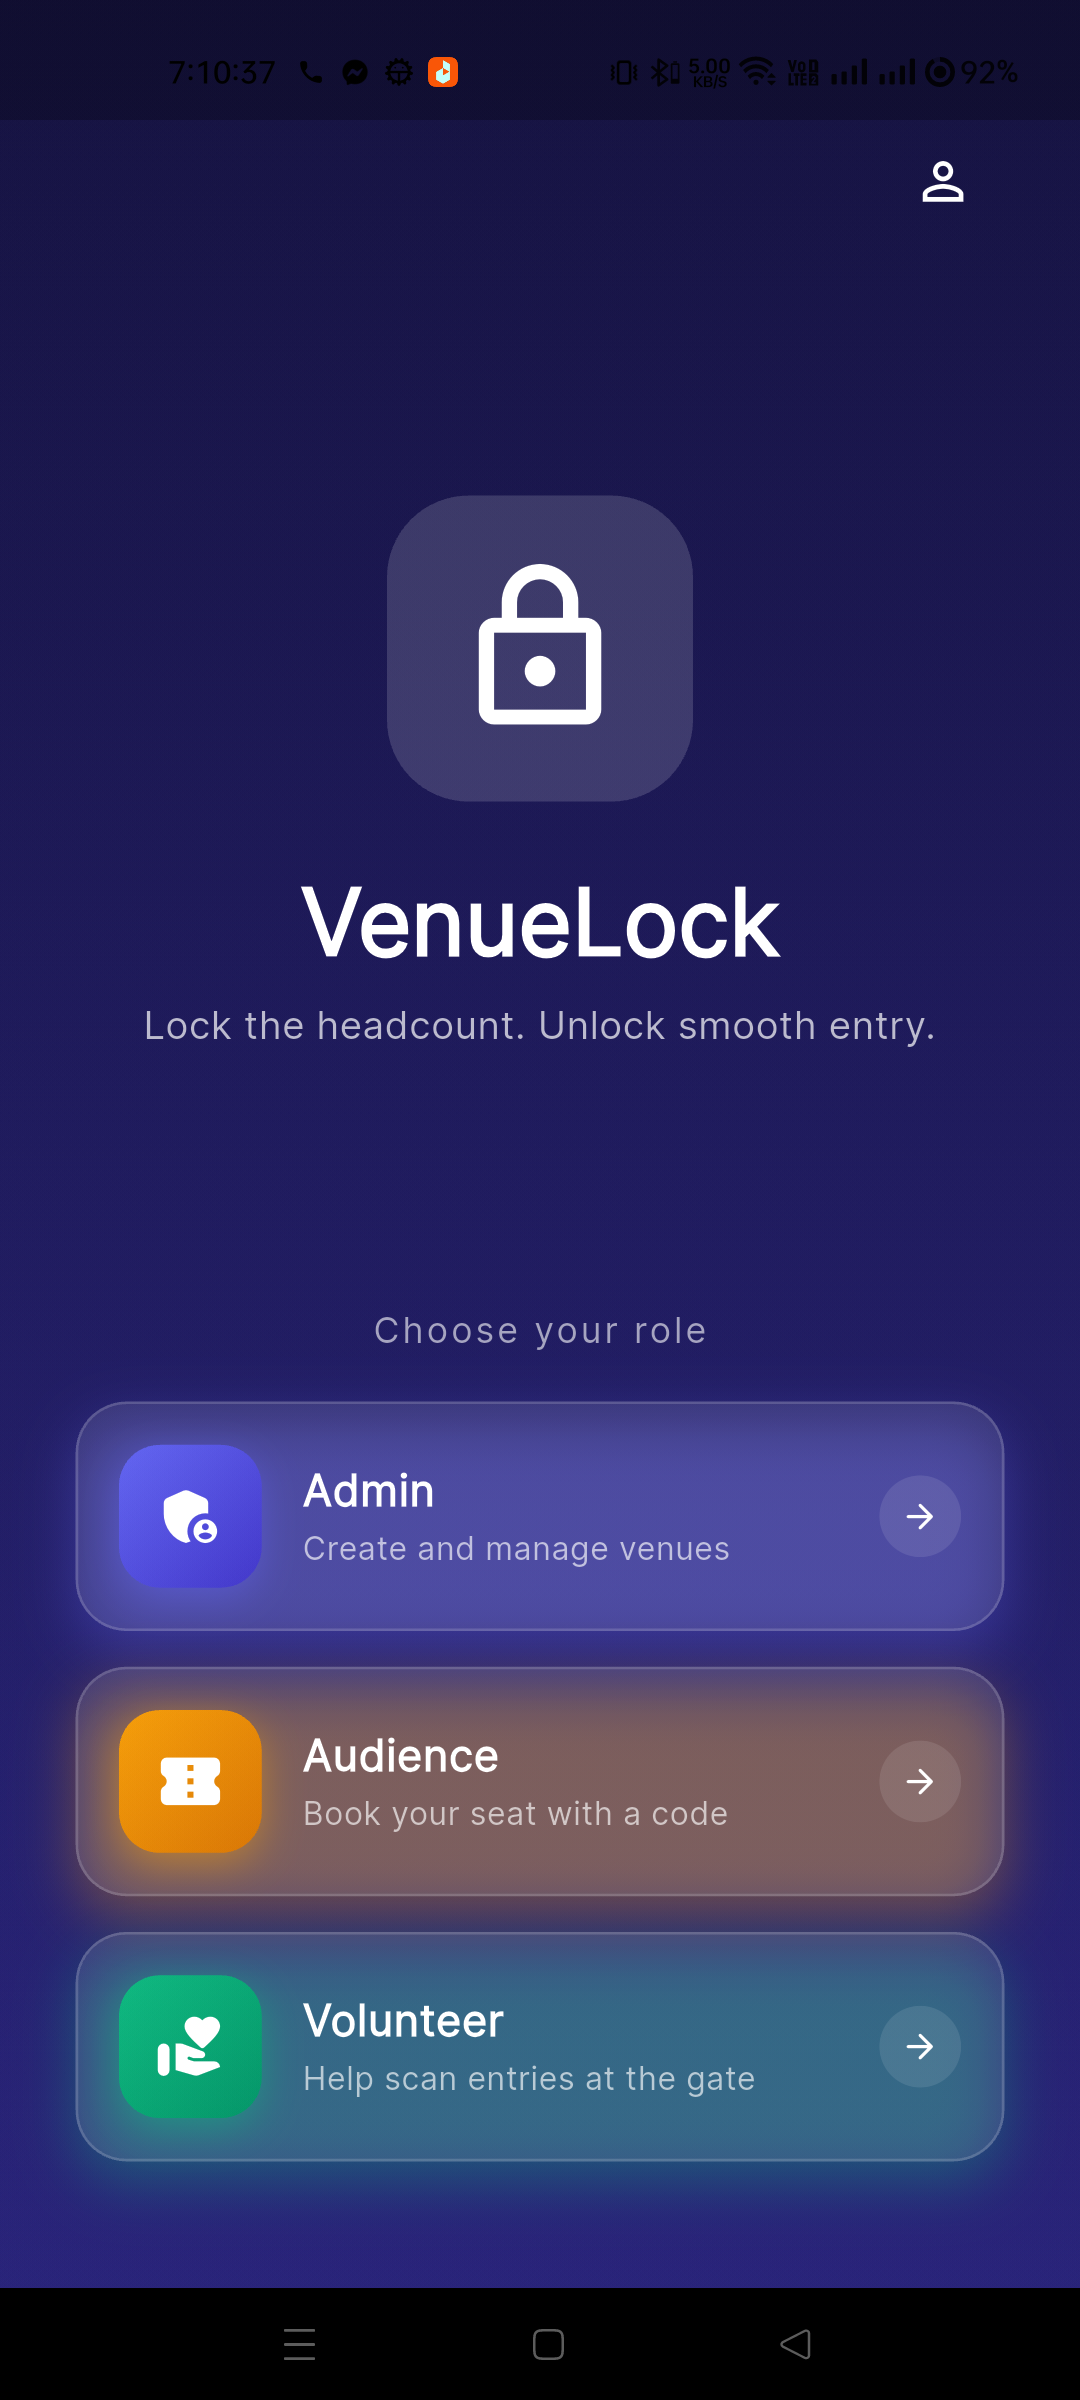
\includegraphics[width=0.31\textwidth]{screenshots/01_role_select.png}
    \hfill
    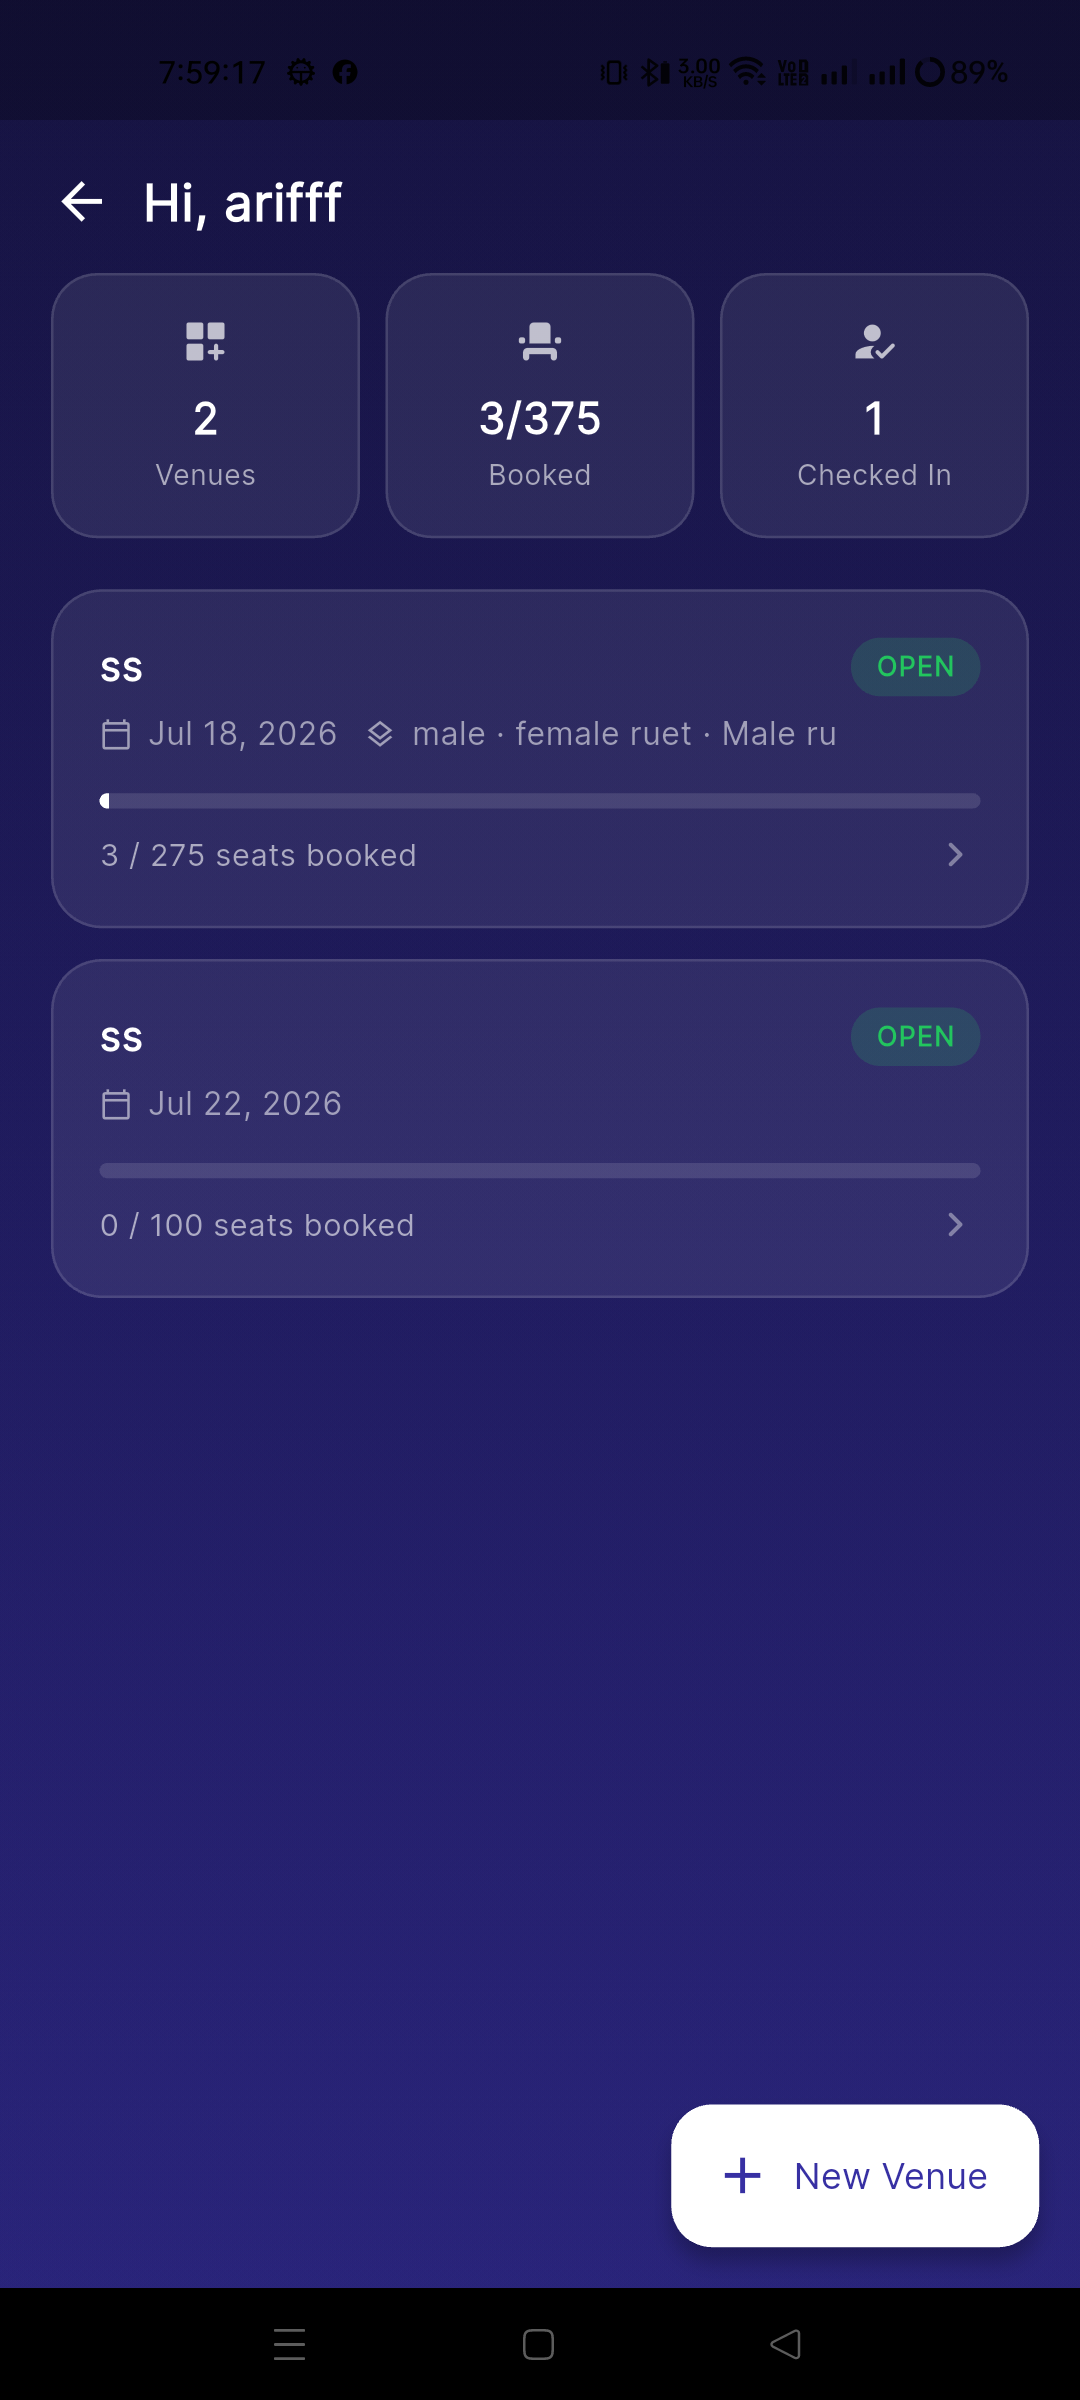
\includegraphics[width=0.31\textwidth]{screenshots/02_admin_dashboard.png}
    \hfill
    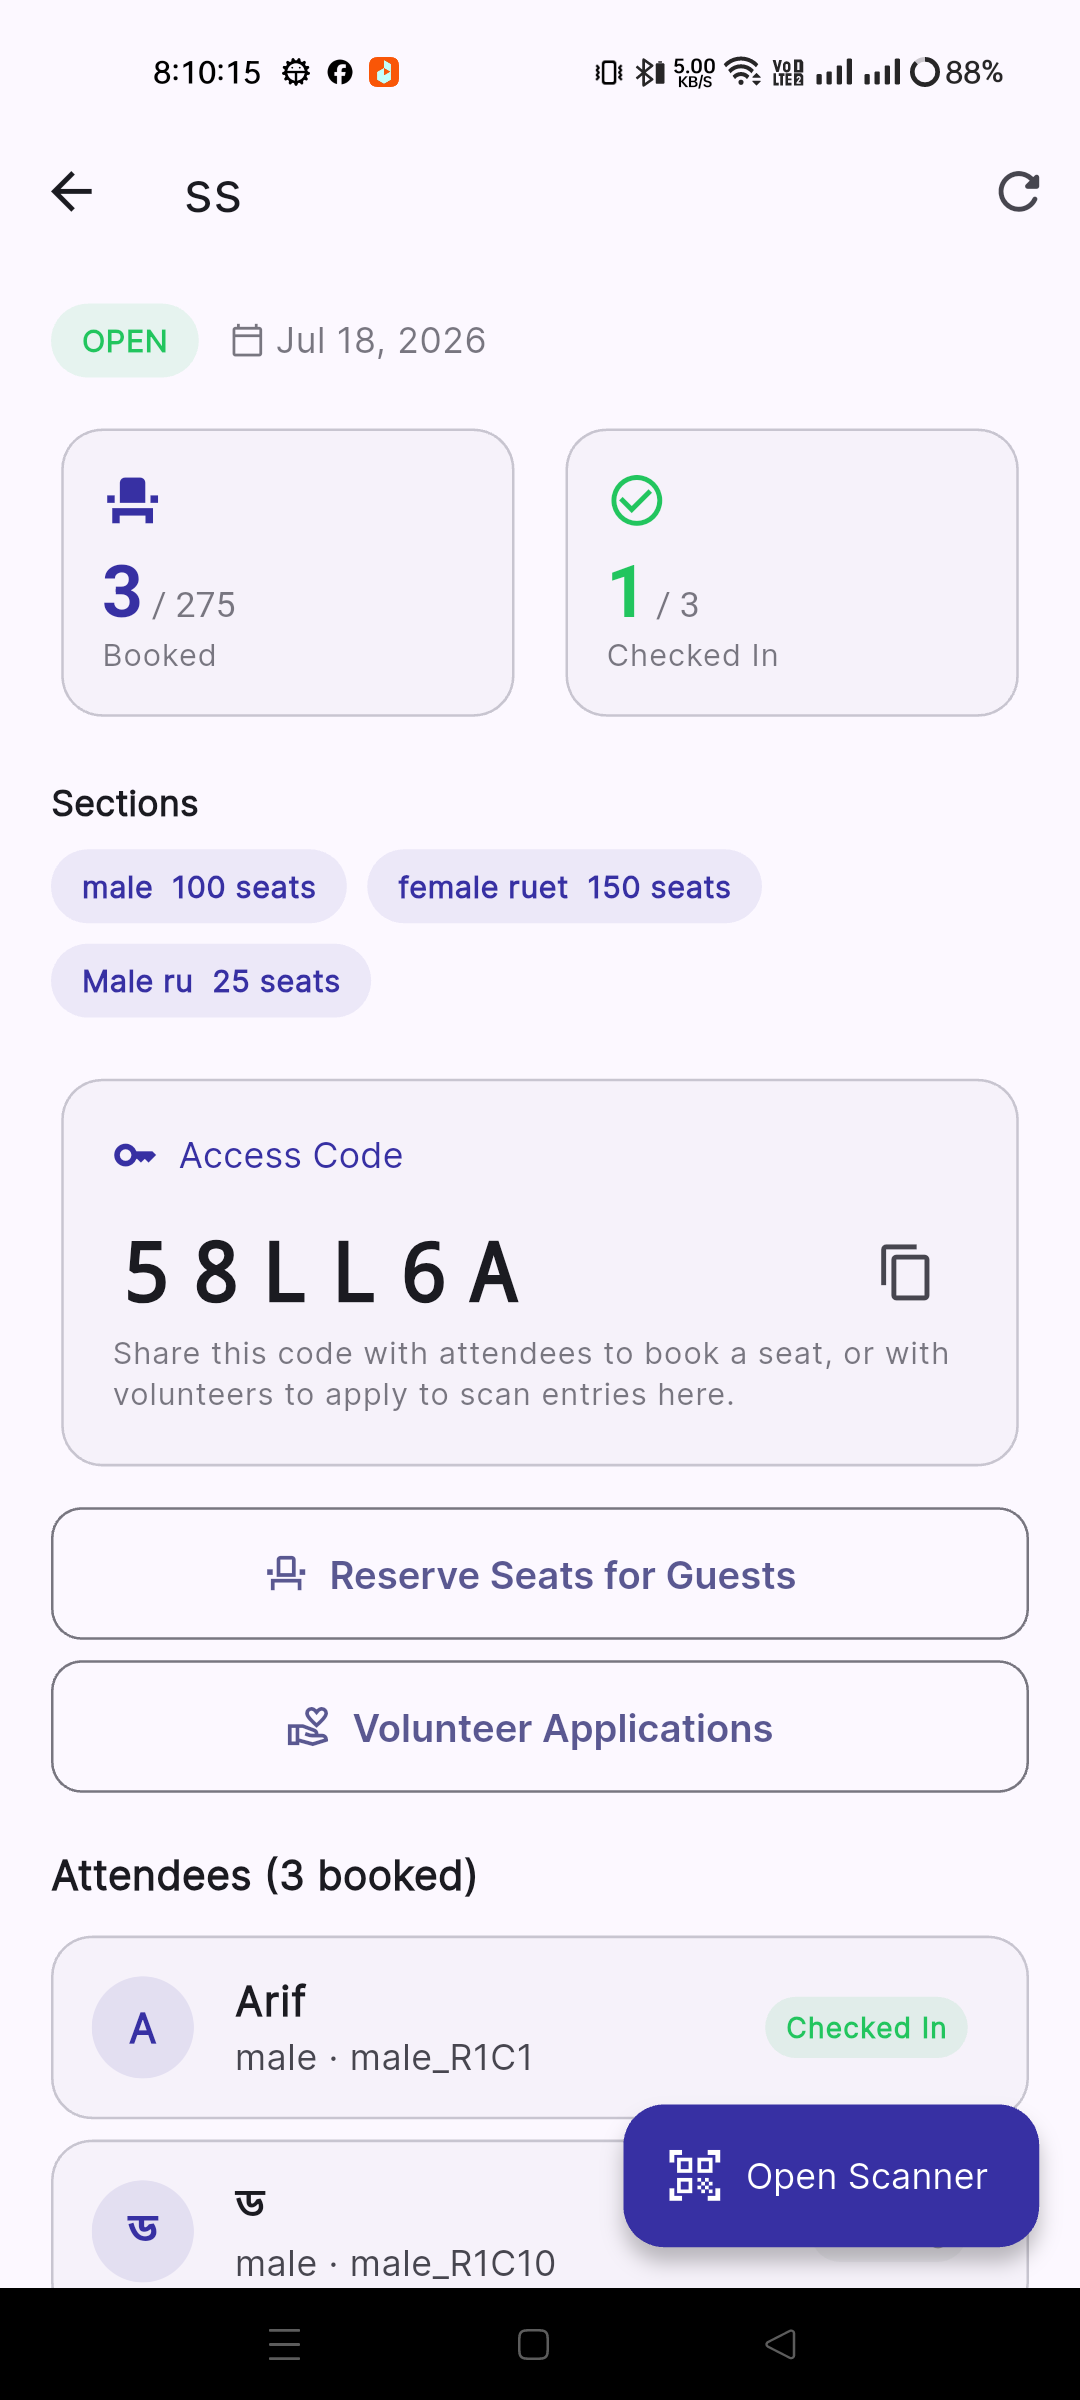
\includegraphics[width=0.31\textwidth]{screenshots/15_venue_detail_populated.png}
    \caption{Role picker, admin dashboard, and a live venue}
\end{figure}

\begin{figure}[H]
    \centering
    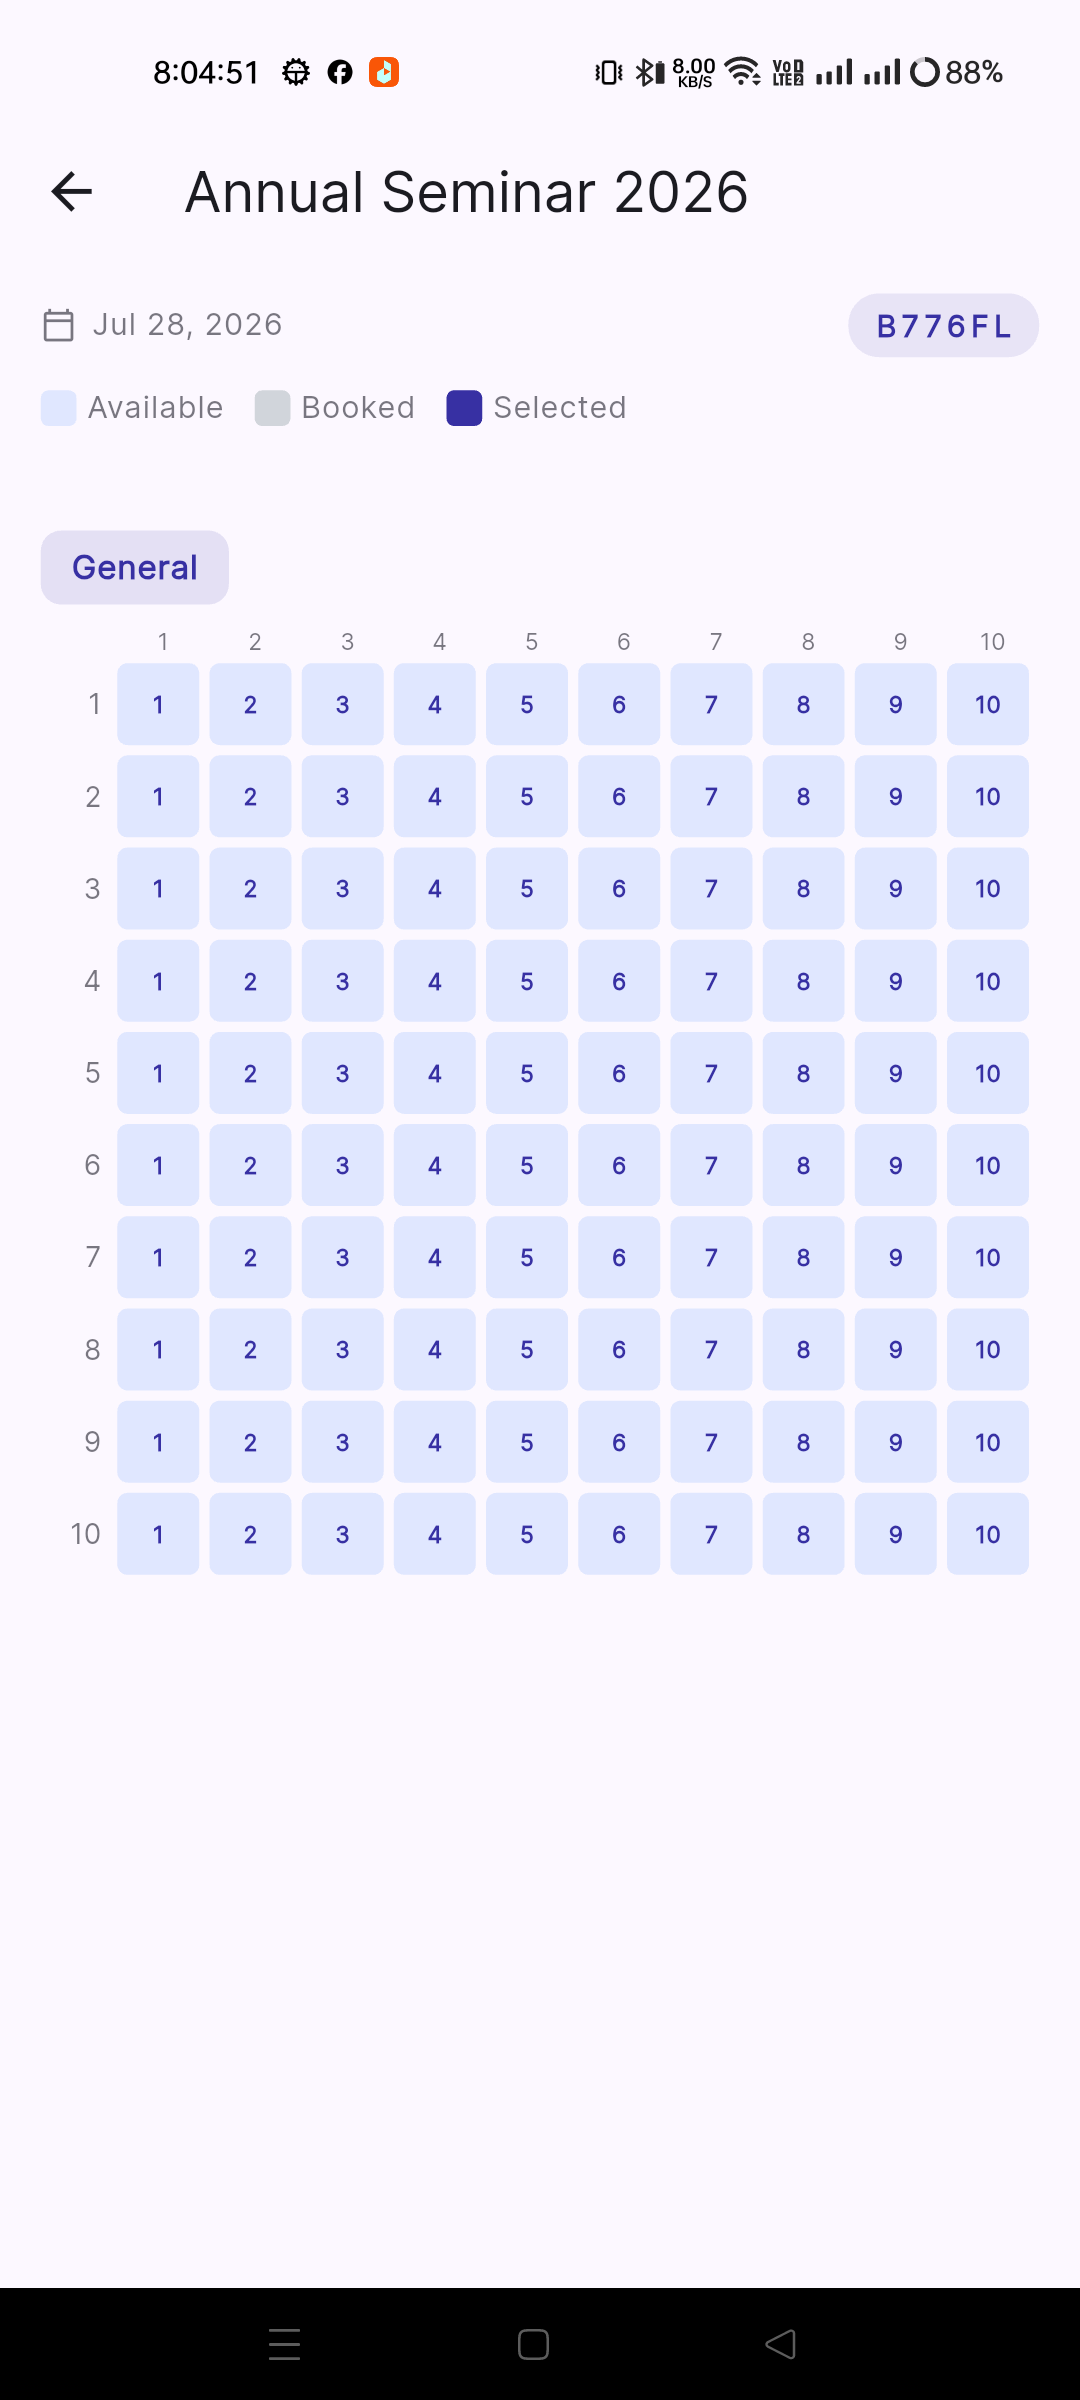
\includegraphics[width=0.31\textwidth]{screenshots/10_audience_seatmap.png}
    \hfill
    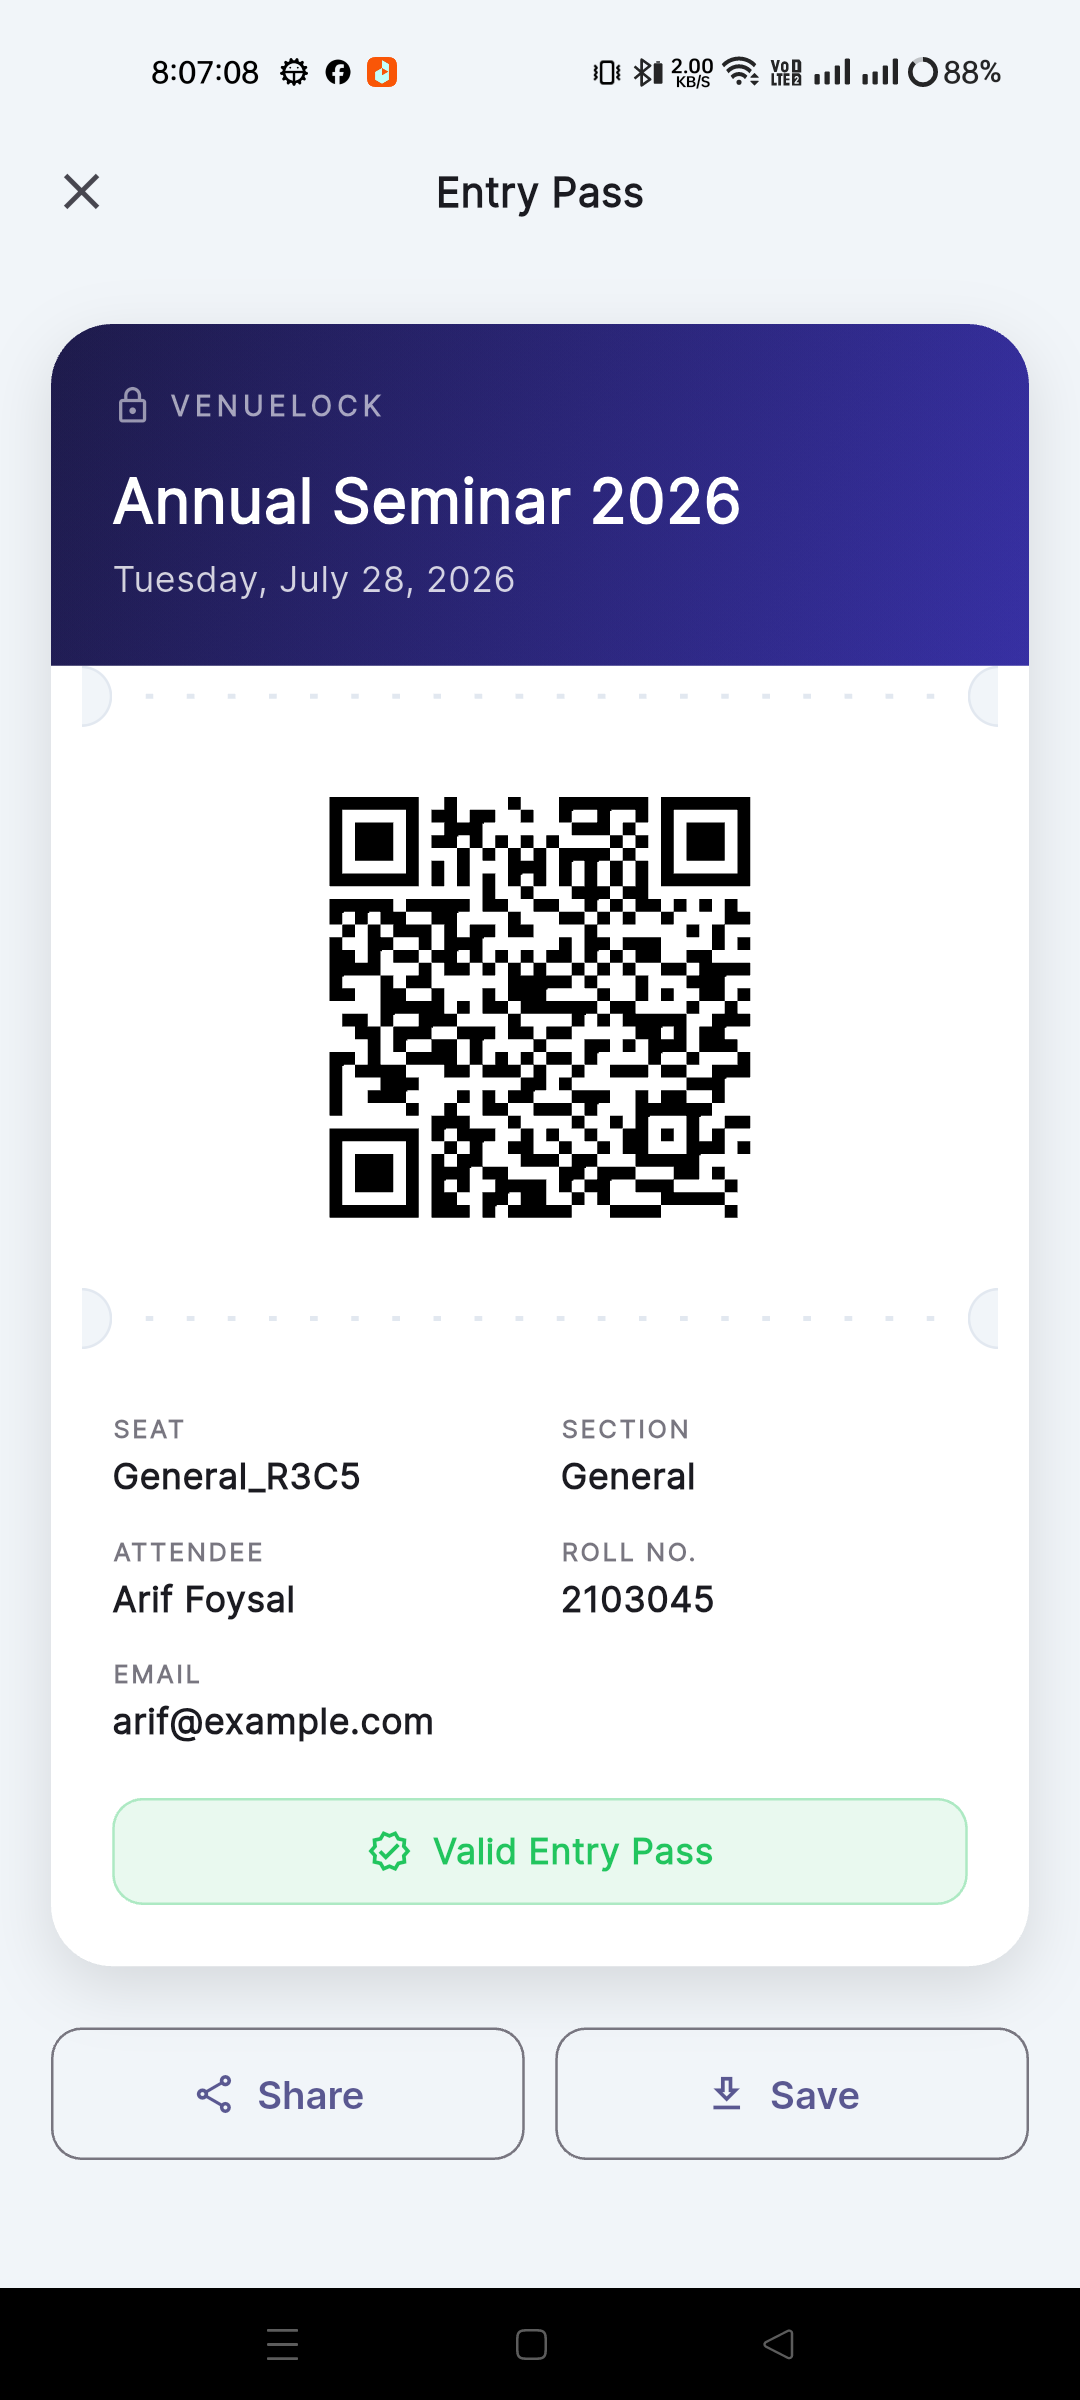
\includegraphics[width=0.31\textwidth]{screenshots/13_entry_pass.png}
    \hfill
    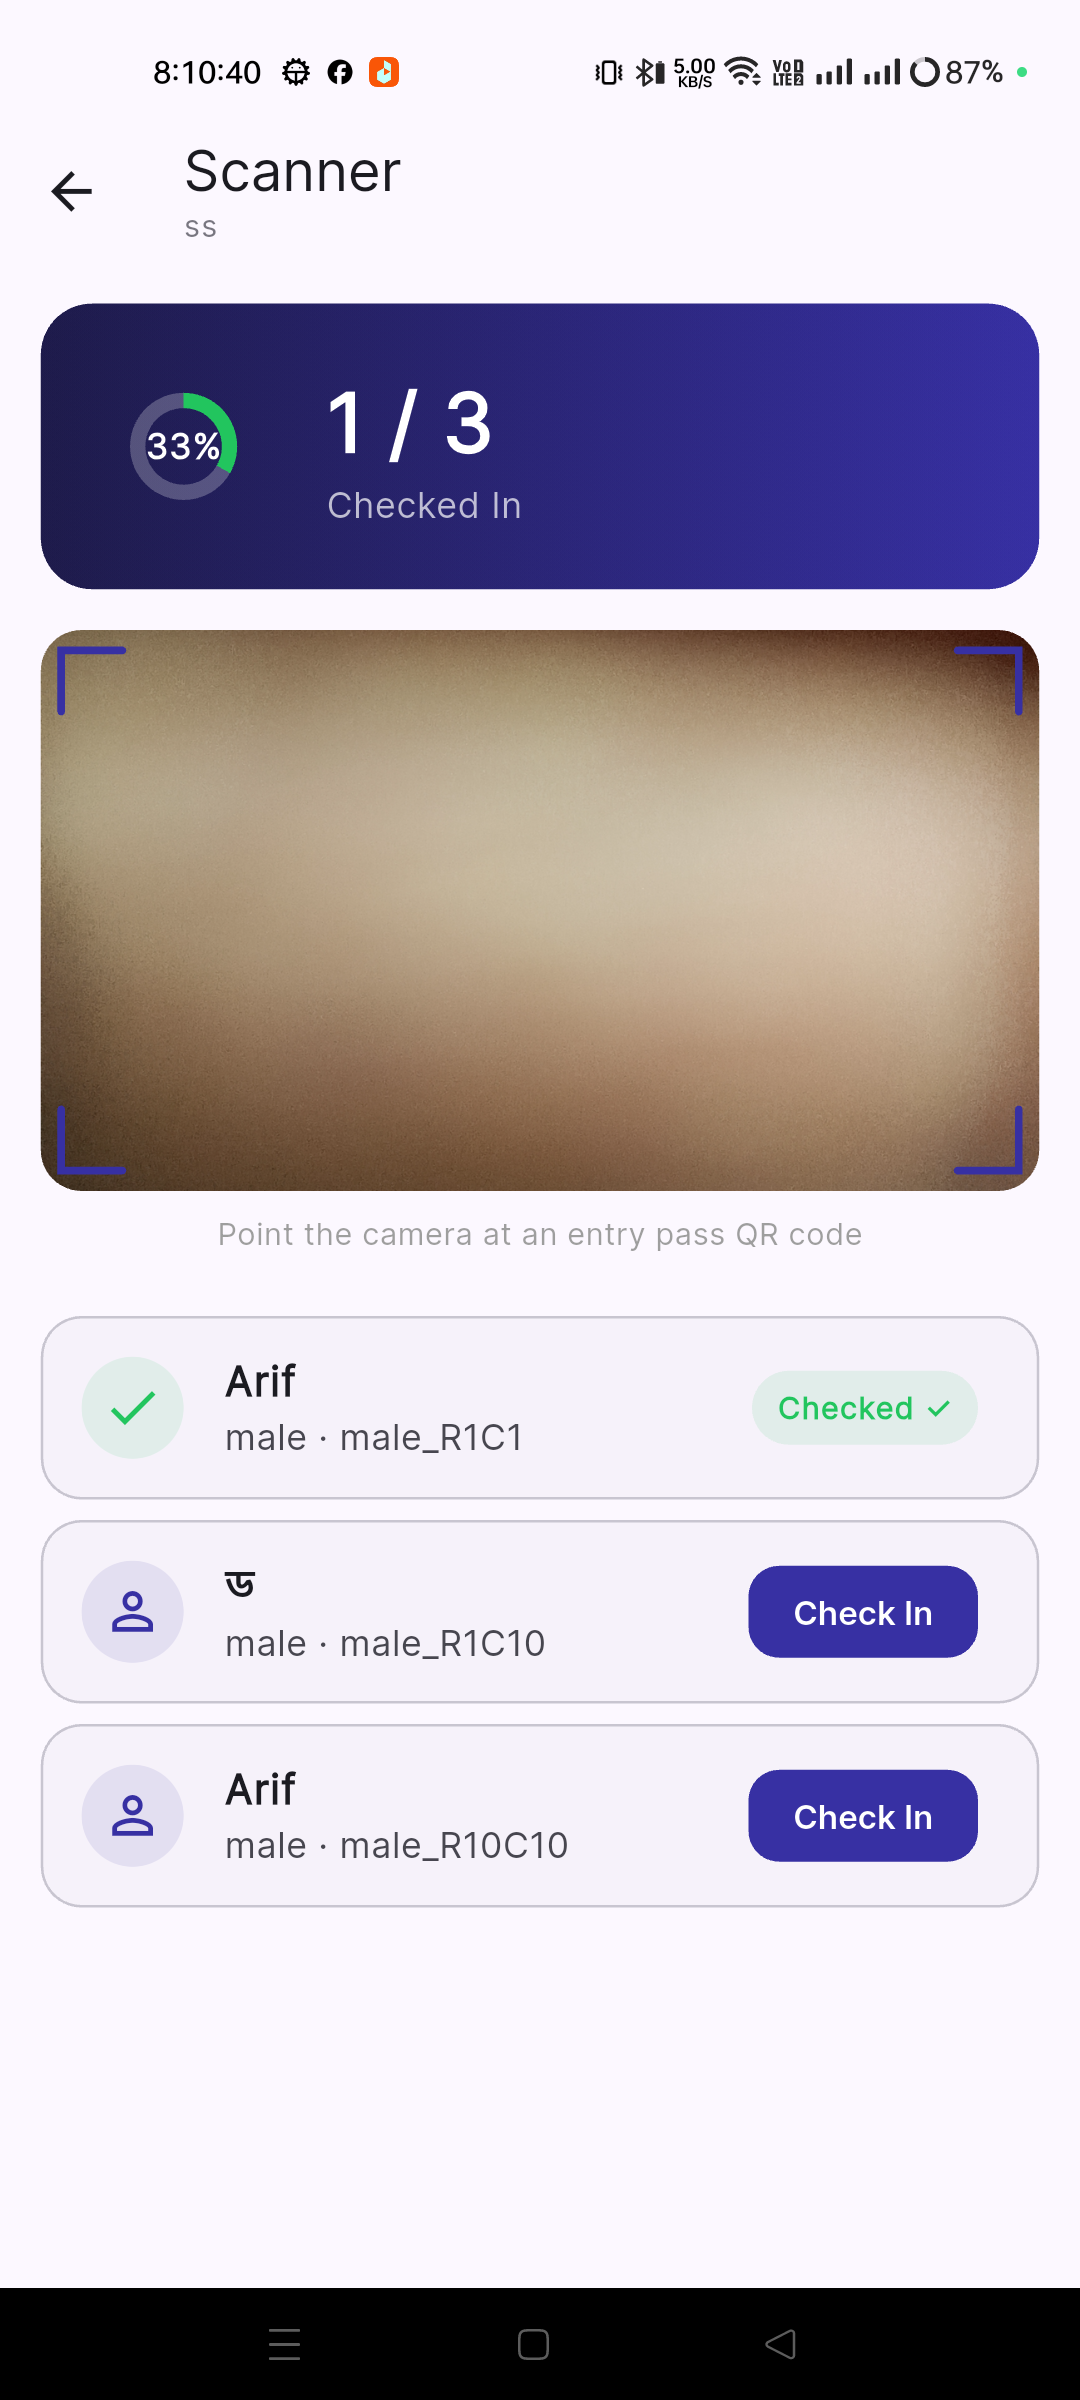
\includegraphics[width=0.31\textwidth]{screenshots/16_scanner.png}
    \caption{Seat map, QR entry pass, and the door scanner}
\end{figure}

% ─────────────────────────────────────────────────────────────
\section{Feature Summary}

\begin{itemize}[leftmargin=1.5em]
    \item Multi-section seat maps (rows $\times$ columns per section) with a
        fixed, server-enforced capacity.
    \item Six-character venue access codes for both attendees and
        volunteers.
    \item Live seat availability, booking progress, and check-in counts.
    \item QR entry passes generated per booking and stored on-device, with
        share and save options.
    \item Camera-based QR check-in with a manual check-in fallback.
    \item Guest seat reservation and release from the admin seat map.
    \item Per-venue, per-device volunteer approval.
    \item Saved profile that prefills booking and volunteer forms.
\end{itemize}

% ─────────────────────────────────────────────────────────────
\section{Technology}

\begin{itemize}[leftmargin=1.5em]
    \item \textbf{App:} Flutter --- \texttt{provider} for state,
        \texttt{go\_router} for navigation, \texttt{mobile\_scanner} for
        camera QR scanning, \texttt{qr\_flutter} for pass generation, and
        \texttt{SharedPreferences} for on-device persistence of the profile,
        saved passes, and volunteer session.
    \item \textbf{Backend:} plain PHP with SQLite, exposed as a small REST
        API. Session-token auth for admins and per-device tokens for
        volunteers; OTP delivery runs through the BDApps carrier SMS/USSD
        SDK.
    \item \textbf{Landing page:} static HTML/CSS/JS, published alongside the
        Flutter web build.
\end{itemize}

% ─────────────────────────────────────────────────────────────
\section{Keywords}

seat booking, event check-in, QR ticket, attendance tracking, venue
management, event organizer, volunteer check-in, seat map, entry pass,
capacity control

% ─────────────────────────────────────────────────────────────
\section{Links}

\begin{itemize}[leftmargin=1.5em]
    \item Live web demo:
        \url{https://theobsidianeye-arif-foysal.github.io/Venue-Lock-v1/}
    \item Android APK:
        \url{https://github.com/TheObsidianEye-ARIF-FOYSAL/Venue-Lock-v1/releases/latest/download/VenueLock.apk}
    \item Source code:
        \url{https://github.com/TheObsidianEye-ARIF-FOYSAL/Venue-Lock-v1}
\end{itemize}

\end{document}
